\documentclass[10pt,a4paper]{article}
\usepackage[utf8]{inputenc}
\usepackage[margin=17mm,top=20mm,bottom=18mm]{geometry}
\usepackage{xcolor}
\usepackage{tabularx,booktabs,array,multirow}
\usepackage{enumitem}
\usepackage{tcolorbox}
\usepackage{tikz}
\usetikzlibrary{arrows.meta,positioning,shapes.geometric}
\usepackage{hyperref}
\usepackage{fancyhdr}
\usepackage{titlesec}
\usepackage{listings}
\pdfmapfile{+cm.map}
\DeclareFontShape{TS1}{cmr}{m}{n}{<-> cmr10}{}

\definecolor{ink}{HTML}{172A42}
\definecolor{deep}{HTML}{10233D}
\definecolor{teal}{HTML}{007B83}
\definecolor{lime}{HTML}{19A598}
\definecolor{pale}{HTML}{EAF6F5}
\definecolor{grey}{HTML}{5D6C7E}
\definecolor{light}{HTML}{F3F6FA}
\definecolor{line}{HTML}{D5E2E8}
\definecolor{amber}{HTML}{A66C10}
\hypersetup{colorlinks=true,linkcolor=teal,urlcolor=teal,pdfauthor={Network Programming Group},pdftitle={ThogaMura - Network Programming Group Proposal}}
\setlength{\parindent}{0pt}
\setlength{\parskip}{4pt}
\setlist[itemize]{leftmargin=*,itemsep=2pt,topsep=2pt}
\setlist[enumerate]{leftmargin=*,itemsep=2pt,topsep=2pt}
\renewcommand{\arraystretch}{1.25}
\titleformat{\section}{\Large\bfseries\color{deep}}{}{0pt}{}
\titleformat{\subsection}{\large\bfseries\color{teal}}{}{0pt}{}
\titlespacing*{\section}{0pt}{7pt}{5pt}
\titlespacing*{\subsection}{0pt}{6pt}{3pt}
\pagestyle{fancy}
\setlength{\headheight}{19pt}
\fancyhf{}
\fancyhead[L]{\footnotesize\bfseries\color{teal} THOGAMURA}
\fancyhead[R]{\footnotesize\color{grey} GROUP PROPOSAL / ASSIGNMENT 02}
\fancyfoot[L]{\footnotesize\color{grey} Draft for team discussion \;$\cdot$\; 15 November 2026}
\fancyfoot[R]{\footnotesize\color{grey} \thepage}
\renewcommand{\headrulewidth}{0.4pt}
\renewcommand{\headrule}{\hbox to\headwidth{\color{line}\leaders\hrule height \headrulewidth\hfill}}

\newtcolorbox{infoBox}[1][]{colback=pale,colframe=line,boxrule=0.6pt,arc=2mm,left=3mm,right=3mm,top=2.5mm,bottom=2.5mm,#1}
\newtcolorbox{plainBox}[1][]{colback=light,colframe=line,boxrule=0.6pt,arc=2mm,left=3mm,right=3mm,top=2mm,bottom=2mm,#1}
\newcommand{\eyebrow}[1]{{\small\bfseries\color{teal}\MakeUppercase{#1}}}
\newcommand{\smalllabel}[1]{{\color{teal}\bfseries #1}}
\newcommand{\quiet}[1]{{\color{grey}#1}}

\lstset{basicstyle=\ttfamily\footnotesize,breaklines=true,frame=single,framerule=0.5pt,rulecolor=\color{line},backgroundcolor=\color{light},showstringspaces=false,xleftmargin=2mm,xrightmargin=2mm,aboveskip=3pt,belowskip=3pt}

\begin{document}

% PAGE 1 --- PURPOSE
\vspace*{7mm}
\eyebrow{Network Programming / Assignment 02}

{\Huge\bfseries\color{deep} ThogaMura}\par
\vspace{2mm}
{\Large\color{teal} LAN-first stock requests and warehouse fulfilment}\par
\vspace{6mm}
\begin{tcolorbox}[colback=deep,colframe=deep,arc=2mm,left=5mm,right=5mm,top=4mm,bottom=4mm]
{\large\bfseries\color{white} The idea in one sentence}\par
{\color{white} A lightweight Java desktop system that helps small distributors request, reserve, pick and dispatch inventory across a local network, with live updates and safeguards against duplicate or competing requests.}
\end{tcolorbox}

\section*{01 \quad The problem}
Small shop and warehouse teams may coordinate stock requests using calls, paper notes or messaging apps. The workflow can break down when two employees request the last available items, staff lose track of pending tasks, or a network interruption makes a submission uncertain. We propose validating these pain points with a real distributor before finalizing the build.

\begin{tabularx}{\linewidth}{>{\bfseries\color{ink}}p{0.22\linewidth} X X}
\toprule
Situation & Typical difficulty & Our focused response \\
\midrule
Concurrent requests & More stock promised than is available & One atomic reservation decision at the server \\
Pending dispatch & Requester and picker have different information & Live notification plus a shared request status \\
Lost response & User cannot tell whether a request was recorded & Request ID, acknowledgement and safe retry \\
Internet outage & Cloud-based workflow may become inaccessible & One local server operating over LAN, without internet \\
\bottomrule
\end{tabularx}

\section*{02 \quad Why this is a suitable university project}
\begin{infoBox}
\textbf{Real workflow + visible networking.} Five members can each own a separate lecture concept: \textbf{TCP, UDP, NIO, multithreading, and TLS}. The application remains one integrated product rather than five unrelated demonstrations.
\end{infoBox}
The Sri Lankan logistics sector has documented challenges involving digital adoption and supply-chain coordination; these findings support investigating the problem, but do not prove demand for this exact product (see references on the final page).

\vfill
\quiet{\textbf{Working title:} ThogaMura combines the Sinhala ideas of stock/wholesale goods (\emph{thoga}) and watch/duty (\emph{mura}). The name is provisional until the group agrees.}\par
\quiet{\textbf{Audience:} Shop counter staff, warehouse pickers and a local supervisor.}\par

\newpage

% PAGE 2 --- WORKFLOW AND ARCHITECTURE
\section*{03 \quad The end-to-end scenario}
\begin{enumerate}
\item A shop client starts and locates the server using \textbf{UDP discovery} (or a manual IP fallback).
\item Staff securely request, for example, \textbf{8 units} of a product using a \textbf{TLS-protected TCP command}.
\item The server checks available stock and \textbf{reserves it atomically}; it returns an acknowledged request ID.
\item A \textbf{Java NIO notification service} signals warehouse clients that something changed.
\item A picker opens the secure request view, marks the request \textbf{PICKED} and then \textbf{DISPATCHED}.
\item All clients can refresh the updated state; an activity record survives a server restart.
\end{enumerate}

\section*{04 \quad Proposed architecture}
\begin{center}
\begin{tikzpicture}[scale=0.91,transform shape,
  font=\small,
  >={Latex[length=2mm]},
  base/.style={rounded corners=2mm,draw=line,thick,align=center,minimum height=12mm,inner sep=3mm},
  client/.style={base,fill=deep,text=white,minimum width=105mm},
  net/.style={base,fill=pale,minimum width=43mm},
  core/.style={base,fill=light,minimum width=93mm},
  conn/.style={->,thick,color=teal}
]
\node[client] (clients) {Java Swing desktop clients\\\footnotesize Shop staff / warehouse pickers / supervisor};
\node[net,below left=12mm and -3mm of clients] (udp) {UDP discovery\\\footnotesize Member 2};
\node[net,below=12mm of clients] (tls) {TLS + TCP commands\\\footnotesize Members 5 + 1};
\node[net,below right=12mm and -3mm of clients] (nio) {NIO change signals\\\footnotesize Member 3};
\node[core,below=18mm of tls] (core) {Concurrent stock reservation service\\\footnotesize ExecutorService + database transactions / Member 4};
\node[base,fill=pale,below=8mm of core,minimum width=60mm] (db) {Embedded persistent database};
\draw[conn] (clients.south west) -- (udp.north);
\draw[conn] (clients.south) -- (tls.north);
\draw[conn] (clients.south east) -- (nio.north);
\draw[conn] (tls.south) -- (core.north);
\draw[conn] (core.south) -- (db.north);
\draw[conn,dashed] (core.east) -| (nio.south);
\end{tikzpicture}
\end{center}

\begin{plainBox}
\textbf{Security boundary.} Product information, authentication and stock-changing commands travel through TLS. The NIO feed sends only a non-sensitive change counter (for example, \texttt{CHANGED:42}); clients then retrieve authorized details through TLS. UDP discovery is a convenience feature, never a trusted identity source.
\end{plainBox}

\subsection*{One small protocol, clear message boundaries}
Use one UTF-8 JSON object followed by a newline per command. TCP delivers bytes, not complete messages, so receivers must buffer until a full line is available. Messages have size limits and request identifiers.
\begin{lstlisting}
{"type":"REQUEST_STOCK","requestId":"r-102","sku":"ITEM-07","quantity":8}
{"type":"ACCEPTED","requestId":"r-102","transferId":"t-027"}
\end{lstlisting}
Repeated submission of \texttt{r-102} must return the original outcome without reserving stock again.

\newpage

% PAGE 3 --- OWNERSHIP
\section*{05 \quad Five-member workload allocation}
\quiet{Each member owns a distinct lecture concept, integration interface, automated tests and a short live demonstration. The assignments below are placeholders until names are added.}\par
\vspace{2mm}

\begin{tcolorbox}[colback=light,colframe=line,arc=1.5mm,boxrule=0.6pt]
\smalllabel{MEMBER 1 \quad TCP communication and reliability}\par
\textbf{Feature:} Stock-request command protocol with acknowledgements, reconnects and safe retries.\par
\textbf{Implement:} Message codec, command client, input validation, read/connect timeouts and request-ID handling.\par
\textbf{Demo:} Submit a request; simulate a lost acknowledgement; retry the same ID without double reservation.\par
\quiet{Lecture link: Socket / ServerSocket, streams, TCP lifecycle, exceptions.}
\end{tcolorbox}

\begin{tcolorbox}[colback=light,colframe=line,arc=1.5mm,boxrule=0.6pt]
\smalllabel{MEMBER 2 \quad UDP server discovery}\par
\textbf{Feature:} Automatically locate ThogaMura on a local network; monitor basic server presence.\par
\textbf{Implement:} DatagramSocket / DatagramPacket discovery, nonce matching, timeout, manual-IP fallback and basic heartbeat.\par
\textbf{Demo:} Launch client without configured address; discover server; show fallback when broadcast is blocked.\par
\quiet{Lecture link: UDP datagrams, ports, timeout, broadcast, InetAddress.}
\end{tcolorbox}

\begin{tcolorbox}[colback=light,colframe=line,arc=1.5mm,boxrule=0.6pt]
\smalllabel{MEMBER 3 \quad Java NIO notifications}\par
\textbf{Feature:} Multiplex a live change-notification feed for several connected clients.\par
\textbf{Implement:} ServerSocketChannel, SocketChannel, Selector, SelectionKey, ByteBuffer, partial read/write handling and disconnection cleanup.\par
\textbf{Demo:} Connect at least 10 clients; one stock change signals all; no one-thread-per-client design.\par
\quiet{Lecture link: NIO channels, selectors, buffer state, non-blocking I/O.}
\end{tcolorbox}

\begin{tcolorbox}[colback=light,colframe=line,arc=1.5mm,boxrule=0.6pt]
\smalllabel{MEMBER 4 \quad Multithreading and safe reservation}\par
\textbf{Feature:} Concurrent request processing without negative or over-promised stock.\par
\textbf{Implement:} ExecutorService, synchronization where appropriate, bounded task handling, atomic database transaction and movement history.\par
\textbf{Demo:} Two simultaneous requests for 8 units when 10 exist; at most one succeeds.\par
\quiet{Lecture link: thread pools, race conditions, shared state, synchronization.}
\end{tcolorbox}

\begin{tcolorbox}[colback=light,colframe=line,arc=1.5mm,boxrule=0.6pt]
\smalllabel{MEMBER 5 \quad Secure sockets and TLS}\par
\textbf{Feature:} Protect authenticated commands and stock information in transit.\par
\textbf{Implement:} SSLServerSocket / SSLSocket, keystore/truststore configuration, certificate validation and basic operator permissions.\par
\textbf{Demo:} Trusted certificate succeeds; untrusted certificate fails; unauthorized write is rejected.\par
\quiet{Lecture link: JSSE, secure sockets, TLS, certificates, authentication/authorization.}
\end{tcolorbox}

\vspace{2mm}
\textbf{Fairness rule:} Each member writes and explains their own module and tests. UI polishing, documentation, integration reviews and bug fixing are shared duties. Avoid assigning a member only presentation or frontend work.

\newpage

% PAGE 4 --- SCOPE AND VERIFICATION
\section*{06 \quad MVP boundaries and correctness rules}
\begin{tabularx}{\linewidth}{>{\bfseries\color{teal}}p{0.18\linewidth} X}
\toprule
Include & Product list and stock balance; stock request; reserve or reject; PICKED and DISPATCHED statuses; request history; live change feed; LAN discovery; trusted TLS commands. \\
\midrule
Defer & Full ERP, accounting, payment processing, purchase orders, suppliers, cloud sync, GPS, AI, complex reporting, barcode hardware and mobile apps. \\
\bottomrule
\end{tabularx}

\begin{infoBox}
\textbf{Invariants to test}\par
\begin{itemize}
\item \texttt{available = onHand - reserved}; available must never fall below zero.
\item Only one result is applied for each unique \texttt{requestId}.
\item A rejected request does not change stock.
\item A dispatched request updates counts and movement history in one transaction.
\item A client can query the latest status after reconnecting; notifications need not be durable.
\end{itemize}
\end{infoBox}

\section*{07 \quad Build plan (suggested 5-week schedule)}
\begin{tabularx}{\linewidth}{>{\bfseries\color{ink}}p{0.15\linewidth} X p{0.31\linewidth}}
\toprule
Period & Joint objective & Exit evidence \\
\midrule
Week 1 & Confirm business scenario, message contract, database schema, repo build and Java version. & Server/client skeleton, protocol spec, green smoke test. \\
Week 2 & Build TCP commands, stock reservations and persistence. & Request accepted or rejected with correct balance. \\
Week 3 & Add UDP discovery, NIO notifications and worker-pool integration. & Multiple clients communicate on a LAN. \\
Week 4 & Add TLS, reconnection behavior, concurrency tests and failure handling. & Verified negative cases, integration suite. \\
Week 5 & Polish Swing UI, run rehearsal, produce report and submission ZIP. & Clean setup, five demos, final PDF. \\
\bottomrule
\end{tabularx}

\section*{08 \quad Technical stack and integration contracts}
\textbf{Server:} Plain Java with Maven, an embedded H2 file database, JSON codec, and JDK networking, security and concurrency APIs.\par
\textbf{Client:} Small Java Swing UI, preceded by console-based network verification.\par
\textbf{Suggested endpoints:} One configurable UDP discovery port, one TLS TCP command port, one read-only NIO notification port.\par
\textbf{Integration rule:} Finalize message types and shared model before parallel coding. Keep command service separate from transport adapters, and store request IDs persistently with a uniqueness constraint.

\subsection*{Must-pass scenarios}
\begin{itemize}
\item Basic create, reserve, pick and dispatch cycle; state survives restart.
\item Two competing reservations cannot oversubscribe stock.
\item Retry after lost response does not create a second reservation.
\item A client reconnects and refreshes state after a missed NIO notification.
\item Invalid JSON, oversized messages, disconnects and timeouts do not crash the server.
\item TLS certificate mismatch rejects the connection; UDP broadcast failure has manual fallback.
\end{itemize}

\newpage

% PAGE 5 --- DEMO, RISKS, HANDOFF
\small
\section*{09 \quad Five-minute group demonstration}
\begin{tabularx}{\linewidth}{>{\bfseries\color{teal}}p{0.12\linewidth} X >{\raggedright\arraybackslash}p{0.26\linewidth}}
\toprule
Order & On-screen action & Presenter \\
\midrule
1 & Client automatically finds the local server. & Member 2 / UDP \\
2 & Client sends a request and receives a unique acknowledgement. & Member 1 / TCP \\
3 & Multiple clients receive an NIO change signal. & Member 3 / NIO \\
4 & Competing requests demonstrate atomic reservation. & Member 4 / Concurrency \\
5 & Secure connection succeeds; untrusted certificate is rejected. & Member 5 / TLS \\
\bottomrule
\end{tabularx}

\section*{10 \quad Risks and safeguards}
\begin{tabularx}{\linewidth}{>{\bfseries\color{ink}}p{0.24\linewidth} X}
\toprule
Risk & Mitigation \\
\midrule
Project becomes a full ERP & Freeze the MVP above; implement networking before adding UI decoration. \\
Module integration breaks & Shared JSON messages, request IDs and model types defined in Week 1. \\
Campus Wi-Fi blocks UDP & Manual server address always available; test on one private hotspot/router. \\
NIO loses partial output & Keep per-client outgoing buffers; register write readiness only while pending. \\
Credentials/data are exposed & TLS for business operations; NIO events expose only a change counter. \\
LAN/server unavailable & State precise limitation: internet-independent, not Wi-Fi- or power-independent. \\
\bottomrule
\end{tabularx}

\section*{11 \quad Submission checklist}
\begin{itemize}[label=$\circ$]
\item Complete project source (client, server, Maven files, tests, example configuration).
\item A \texttt{README} with exact commands for building and running on two devices.
\item A single PDF report: problem, architecture, five contributions, screenshots, test results, limitations.
\item Evidence of independent implementation (module ownership, commits, feature demonstration).
\item Both project and report placed in \textbf{one ZIP}; only one group member uploads to Moodle.
\end{itemize}

\begin{plainBox}
\textbf{Decisions required at the first team meeting}\par
\begin{enumerate}
\item Confirm this idea with the lecturer and at least one potential shop/warehouse user.
\item Assign the five named owners and agree on the available weeks.
\item Choose JDK version and whether the demo uses one laptop or multiple LAN devices.
\item Freeze the MVP before adding any optional features.
\end{enumerate}
\end{plainBox}

\vspace{0mm}
{\footnotesize\color{grey}\textbf{Research basis}\par
[1] World Bank, \emph{Sri Lanka Systematic Country Diagnostic Update}, sections on logistics and digital adoption (2022).\par
[2] World Bank, \emph{Sri Lanka's Economy Reaches Pre-Crisis Levels but Recovery Uneven} (October 2026), digital traceability and logistics.\par
[3] Oracle, Java SE 25 API documentation for \texttt{DatagramSocket}, \texttt{Selector}, \texttt{SocketChannel}, \texttt{SSLSocket}, and \texttt{SSLServerSocket}.\par
This is a design proposal, not evidence of completed code or validated customer demand.}
\normalsize

\end{document}
